\chapter{Estado del arte}

% **************************** Define Graphics Path **************************
\graphicspath{{Chapter2/Figs/}}

\section{Software Defined Networking}
Aspectos generales
%https://www.necam.com/docs/?id=2709888a-ecfd-4157-8849-1d18144a6dda

%http://www.iaria.org/conferences2014/filesICNS14/InfoSys%202014%20Control%20Plane%20Scalability%20in%20SDN-%20%20v1.2.pdf

%http://arxiv.org/pdf/1408.6760.pdf

%Ventaja encontrada: puede reducir el procesamiento que se debe hacer en los dispositivos, y eso reduce costos operacionales y aumenta el rendimiento de la red.
%%OPEN promises to reduce the Total Cost of Ownership of  various network  infrastructures  in  part  by  simplifying  the  datapath  switches;  it  provides  greater  control  to  the  operator  to customize and optimize their networks for the features they need and the services they provide; and finally it allows innovation to take place at a much faster rate, by  helping the network evolve  more rapidly in software (implemented outside-the-box), with possibly greater diversity of solutions generated by a larger pool of developers.
%%In today’s packet switched networks, a router is  both  the  control  element  which  makes  control  decisions  on  traffic routing,  as  well  as  the  forwarding element  responsible  for forwarding packets,  and  both  these  functionalities  are tightly linked (Fig.  1a). Housing  control and data functions in the same box necessarily complicates the equipment, which aside from making routing decisions and switching packets, also needs to have all the intelligence necessary for  aggregating  and  disseminating  routing  information, using fully  distributed  routing protocols like OSPF or IS-IS. Furthermore, in IP/MPLS networks, another layer of complexity is added with the need for distributed signaling and label  distribution mechanisms like  RSVP-TE and LDP. Within  a  domain,  an  IP/MPLS  network  may additionally support a host of other protocols such as iBGP, RIP, LMP, SNMP and MP-BGP together  with  many  more protocols for multicast and IPv6. All of these features contribute to control plane load, increased fragility and increased cost (FUENTE: el parrafo anterior y este son del ultimo paper de las vpns sobre SDN)

\section{OpenFlow}
Aspectos generales
%http://article.sciencepublishinggroup.com/pdf/10.11648.j.ajsea.20140306.12.pdf

%http://www.spirent.com/~/media/White%20Papers/Broadband/PAB/OpenFlow_Performance_Testing_WhitePaper.pdf

\section{Open vSwitch}
%http://openvswitch.org/pipermail/discuss/2012-February/006447.html

%http://openvswitch.org/support/dist-docs/ovs-vswitchd.8.txt

%http://benpfaff.org/papers/ovs.pdf

%http://networkheresy.com/2014/11/13/accelerating-open-vswitch-to-ludicrous-speed/

%http://bluesy.wang/notes/2014/09/14/flow-caching-for-high-entropy-packet-fields/

%http://yuba.stanford.edu/~nickm/papers/flow-caching.pdf

%http://wangcong.org/2012/10/20/an-overview-of-openvswitch-implementation/

%https://www.google.com/url?sa=t&rct=j&q=&esrc=s&source=web&cd=1&ved=0ahUKEwixpuyBieLLAhUCdR4KHVV7CKgQFggfMAA&url=https%3A%2F%2Fnsrc.org%2Fworkshops%2F2014%2Fnznog-sdn%2Fraw-attachment%2Fwiki%2FAgenda%2FOpenVSwitch.pdf&usg=AFQjCNFg9VULvEmHMXQAsuTOE6XLH6WbzQ&bvm=bv.117868183,d.dmo&cad=rja

%http://openvswitch.org/slides/OpenStack-131107.pdf

%http://openvswitch.org/slides/openvswitch.en-2.pdf

%https://www.google.com/url?sa=t&rct=j&q=&esrc=s&source=web&cd=3&ved=0ahUKEwjP95D9ieLLAhVIpB4KHUKeCzYQFggoMAI&url=http%3A%2F%2Fopenvswitch.org%2Fsupport%2Fovscon2014%2F17%2F1530-ovsconf2014_chadnorgan.pptx&usg=AFQjCNEmnrXDB0psj5oXvoAzVYr8F5sLtQ&cad=rja

%https://www.google.com/url?sa=t&rct=j&q=&esrc=s&source=web&cd=1&cad=rja&uact=8&ved=0ahUKEwjZvdvaiuLLAhWF1h4KHfYrCKoQFggiMAA&url=http%3A%2F%2Fopenvswitch.org%2Fsupport%2Fovscon2014%2F18%2F1600-ovs_perf.pptx&usg=AFQjCNGGTT0rHmENeZ2ZcoRfWNFJ__hBLw

\section{Multiprotocol Label Switching (MPLS)}
Conceptos básicos

\section{Red Privada Virtual (VPN)}
Conceptos básicos

\section{Aplicaciones de SDN}
El paradigma SDN, por definición, está basado en el software. Esto implica que el rango de aplicaciones o modos de uso que se le puede dar al paradigma es enorme. En esta sección se estudiarán algunas aplicaciones existentes sobre SDN, haciendo foco en la implementación de redes privadas virtuales, debido a que es el servicio que provee RAUFlow.
\subsection{Implementación de VPNs}
El desarrollo de redes privadas virtuales (VPN) es un tema de investigación relativamente común en SDN, ya que es un servicio de gran demanda en el mundo actual. A continuación se estudiarán algunas implementaciones existentes de VPN sobre SDN. \\ \\
\textbf{Proyecto CoCo} \\
CoCo \cite{coco-paper} es un proyecto que estudia el desarrollo de un servicio de VPN multipunto enfocado hacia investigadores, para permitirles intercambiar información de modo confiable y seguro. Uno de sus principales enfoques es la facilidad de uso, lo cual es una ventaja frente a las implementaciones tradicionales (no SDN) de este servicio. Sólo requiere que el administrador haga una configuración inicial de la red, y luego los usuarios finales pueden crear, modificar y  eliminar VPNs a demanda mediante un portal web. \\ \\
\begin{figure}[t]
	\caption{Arquitectura de CoCo. Imagen extraída de \cite{coco-paper}}
	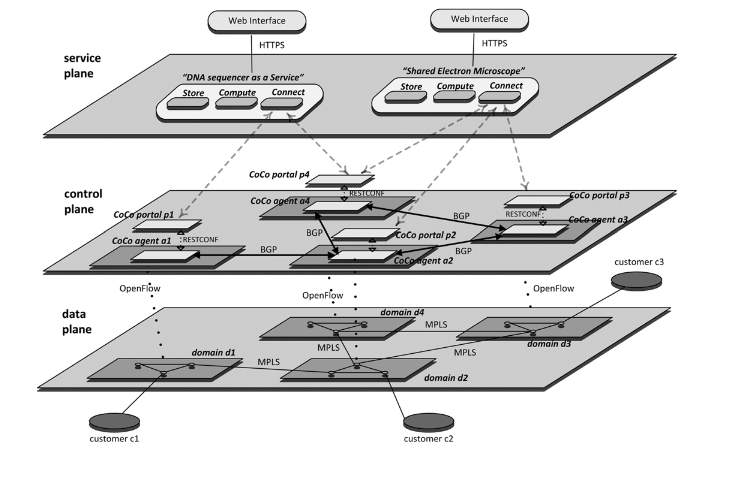
\includegraphics[scale=0.65]{coco_imagen}
	\centering
	\label{fig:coco_imagen}
\end{figure}
La arquitectura de CoCo, que se ilustra en la figura \ref{fig:coco_imagen}, está diseñada para aplicarse a muchos dominios. Cada dominio es una red OpenFlow administrada por un controlador OpenDaylight, llamado agente CoCo. Este último tiene dos grandes tareas. La primera es controlar los switches OpenFlow de su dominio, haciendo descubrimiento de la topología y configurando las reglas de reenvío de los switches. La segunda tarea es en el plano de control de la arquitectura, y consiste en utilizar el protocolo BGP para intercambiar información de accesibilidad con otros agentes CoCo (por ende, otros dominios). \\ \\
Como ya se mencionó, la red de cada dominio está compuesta por switches OpenFlow. Éstos últimos pueden ser internos o de borde, también llamados Provider Edge (o PE). Los de borde son los que se conectan con otros dominios o con las redes cliente (Customer Edge). Las reglas de reenvío están basadas en MPLS, y se utilizan dos niveles de etiquetas. La etiqueta exterior sirve para identificar al switch PE al cual se debe enviar un paquete. La etiqueta interior identifica a la VPN a la cual pertenece el paquete. Esto quiere decir que el tráfico que se recibe por la red CE es etiquetado apropiadamente por el switch PE que recibe dicho tráfico. Cuando el tráfico sale de la red interna hacia la red CE, el switch PE se encarga de remover las etiquetas MPLS del tráfico saliente. \\ \\
\textbf{OpenFlow para mejorar la escalabilidad de un servicio IP-VPN} \\
En \cite{ip-vpn-bgp-sdn} se estudia el problema de la escalabilidad al proveer un servicio de IP-VPN, y propone una solución basada en SDN y OpenFlow. Si un proveedor de servicios de telecomunicaciones ofrece un servicio de IP-VPN, es posible que lo haga utilizando el protocolo BGP. Dicho protocolo se utiliza para intercambiar la información de ruteo correspondiente a cada red cliente conectada al servicio. En un esquema no SDN, el procesamiento del plano de control (en este caso BGP) queda a cargo de los routers de la red. Esto presenta un posible problema de escalabilidad. Cuando se agregan nuevos clientes a la VPN, la nueva información de ruteo debe ser propagada. Los recursos de CPU y memoria de los routers serán consumidos de acuerdo a lo que exijan los nuevos clientes. Por lo tanto, es necesario confirmar que hay margen en la capacidad de los dispositivos antes de aceptar nuevos clientes. \\ \\
La solución que se propone para atacar este problema es utilizar OpenFlow. Se despliega un controlador OpenFlow que además ejecuta múltiples demonios BGP, uno por cada cliente. Los demonios BGP se encargan del intercambio de información de ruteo con los routers de las redes cliente. Un cliente puede tener múltiples redes conectadas a la VPN. Cuando el controlador recibe información de ruteo correspondiente a una determinada red, el demonio BGP encargado de ese cliente notifica a las demás redes del mismo cliente. Además, la misma información de ruteo recibida es procesada para generar las reglas de forwarding (entradas de flujos en los switches OpenFlow) que aseguren la conectividad. Dado que distintos clientes pueden compartir direcciones IP, es necesario que la red OpenFlow pueda distinguir de algún modo a qué cliente pertenece el tráfico. Esto lo logra asignando etiquetas de VLAN a los paquetes cuando entran a la red, que identifican a cada cliente. En el trabajo se menciona, como objetivo futuro, utilizar MPLS en lugar de etiquetas de VLAN. \\ \\
Con la utilización de OpenFlow se resuelve en gran medida el problema de la escalabilidad, ya que se saca el procesamiento del protocolo BGP de los routers y se concentra todo en el controlador. Si bien agregar nuevos clientes a la VPN aumentará la carga de procesamiento y memoria, el controlador puede manejarlo más fácilmente que los dispositivos de red, que tienen recursos mucho más limitados. \\ \\
\textbf{SDxVPN} \\
SDxVPN \cite{sdxvpn} es una propuesta de implementación de VPNs de capa 2 y 3, basadas en MPLS y OpenFlow. Intenta atacar tres problemáticas comunes que experimentan los proveedores de servicios al ofrecer VPNs: 1) complejidad en la administración de las VPNs, 2) los dispositivos de red deben implementar un plano de control muy complejo, y eso los encarece, y 3) ejecutar el plano de control en los dispositivos puede ser muy costoso para el rendimiento cuando aumenta la cantidad de clientes, y esto presenta un problema de escalabilidad. \\ \\
\begin{figure}[t]
	\caption{Diseño de SDxVPN. Imagen extraída de \cite{sdxvpn}}
	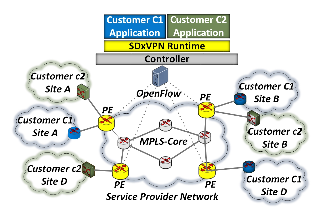
\includegraphics[scale=1.00]{sdxvpn_architecture}
	\centering
	\label{fig:sdxvpn_architecture}
\end{figure}
\begin{figure}[t]
	\caption{Modo de operación de cada servicio de acuerdo a su capa. Imagen extraída de \cite{sdxvpn}}
	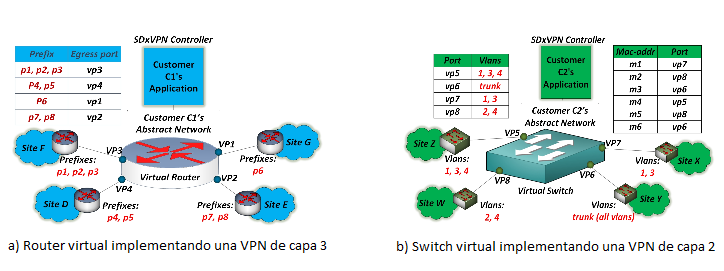
\includegraphics[scale=0.65]{sdxvpn_design}
	\centering
	\label{fig:sdxvpn_design}
\end{figure}
El diseño de la solución propuesta se puede ver en la figura \ref{fig:sdxvpn_architecture}. En la misma se observa la red de un hipotético proveedor de servicios conectada a dos clientes, cada uno con tres redes. La red del proveedor está dividida en dos partes: la región \textit{core} y los routers PE (Provider Edge). Este trabajo argumenta la necesidad enfoques híbridos SDN/Legacy, y es aquí donde lo aplica: si bien los routers PE son OpenFlow, el core de la red no utiliza SDN, y depende de LDP y Quagga para la distribución de etiquetas MPLS. Esto implica que los routers PE, además de utilizar OpenFlow, deben implementar Quagga y LDP. \\ \\
Otro dato importante que muestra la figura \ref{fig:sdxvpn_architecture} es la utilización de una aplicación por cada cliente. Esto permite proveer a los clientes un control personalizado sobre su servicio de VPN. Esas aplicaciones corren sobre una visión abstracta de la red, que depende de la capa del servicio. Si la VPN es de capa 3, el controlador SDxVPN ofrece un router virtual, y si es de capa 2 ofrece un switch virtual. Cada puerto en uno de estos dispositivos virtuales representa un puerto real de un dispositivo PE con un dispositivo CE (Customer Edge). Este enfoque le ofrece al cliente una visión abstracta de la red del proveedor, y se puede ver en la figura \ref{fig:sdxvpn_design}. En el caso de una VPN de capa 3, el cliente debe elegir un mecanismo de ruteo. Para el caso que muestra la figura, puede alcanzar con ruteo estático, pero para casos más complejos, el router virtual puede utilizar Quagga como motor. Todo esto implica que se construirá una tabla de ruteo virtual, la cual será traducida a flujos OpenFlow en los dispositivos PE. \\
Para la VPN de capa 2, el cliente debe asociar cada puerto del switch virtual con un conjunto de identificadores de VLAN. A ese mapeo se suma un mecanismo para aprender direcciones MAC (ya que debe comportarse como un switch de capa 2), y todo esto (igual que en la VPN de capa 3) se traduce en flujos OpenFlow que serán instalados en los dispositivos PE.

%http://yuba.stanford.edu/~nickm/papers/ofc11-saurav-mpls.pdf y http://klamath.stanford.edu/~nickm/papers/mpls-sigcomm11.pdf
\subsection{Otras aplicaciones}
En la sección anterior se presentaron algunas implementaciones de VPNs en SDN, que es la aplicación de más interés en este trabajo. A continuación se listan otras aplicaciones que se le puede dar a OpenFlow y SDN.
\begin{itemize}
	\item \textbf{Ingeniería de tráfico} es una disciplina que tiene como objetivo principal optimizar el rendimiento de una red. Una parte crucial de esta disciplina es poder monitorear en tiempo real el estado de cada elemento de la red. Esto es algo que OpenFlow resuelve, ya que puede registrar estadísticas por cada flujo, en tiempo real. Por ejemplo, en \cite{opennetmon} se presenta OpenNetMon, un módulo open source para el controlador POX que aprovecha las capacidades de monitoreo de OpenFlow y hace disponibles todas esas estadísticas para las aplicaciones que corren sobre el controlador. Una aplicación luego puede utilizar ese módulo y todas las estadísticas que provee para hacer ingeniería de tráfico, y tratar de optimizar los recursos de la red. \\
	El manejo de los flujos para lograr load balancing y la tolerancia a fallas son otros enfoques importantes, partes de la ingeniería de tráfico en SDN. En caso de que el lector desee profundizar en este tema, se recomienda la lectura de \cite{roadmap-sdn-te}, que hace un estudio completo de los enfoques actuales para la ingeniería de tráfico en redes OpenFlow.
	\item \textbf{Quality of Service}. Un problema muy común hoy en día es el de proveer distintos niveles de calidad de servicio, y SDN puede ser utilizado con ese propósito. El objetivo es aplicar distintos niveles de servicio a un determinado tráfico de acuerdo al cliente o al tipo de aplicación al que pertenece. Para lograr eso se pueden aplicar mecanismos como la reserva de recursos y el enrutamiento dinámico para cada flujo. \\
	Algunos ejemplos de trabajos hechos en este campo son: 1) FlowQoS \cite{flowqos}, una herramienta que permite a redes hogareñas reservar ancho de banda para cada tipo de tráfico mediante OpenFlow, 2) un framework basado en EuQoS \cite{euqos} para redes a gran escala, que utiliza OpenFlow para asignar prioridades a demanda a flujos de clientes. \\
	Si el lector desea profundizar en el tema de QoS sobre SDN, se recomienda la lectura de \cite{survey-sdn-qos}.
	\item \textbf{Detección y mitigación de ataques DoS}. Un controlador OpenFlow podría aprovechar las métricas y estadísticas ofrecidas por los switches OpenFlow para detectar, en tiempo real, ataques de denegación de servicio. El controlador también podría reaccionar ante el ataque, aplicando las entradas de flujos que correspondan para bloquear el tráfico utilizado, y así mitigar el efecto del ataque. Por ejemplo, Dossy \cite{openflow-dos-dossy} es una aplicación que corre sobre el controlador Beacon y permite detectar y mitigar ataques DoS. Analiza los mensajes packet\_in que recibe y las estadísticas de los flujos para detectar los ataques, y una vez los detecta, instala flujos para bloquear el tráfico atacante.
\end{itemize}

\section{Simuladores y emuladores}
\subsection{DOT} %es distribuido, asi que no aplicaria mucho, pero esta bueno, asi que capaz que si
\subsection{Estinet} %si
\subsection{fs-sdn} %si
\subsection{Mininet} %si
Mininet es un emulador de redes SDN que permite emular hosts, switches, controladores y enlaces. Utiliza virtualización basada en procesos para ejecutar múltiples instancias (hasta 4096) de hosts y switches en un unico kernel de sistema operativo. También utiliza una capacidad de Linux denominada \textit{network namespace} que permite crear "interfaces de red virtuales", y de esta manera dotar a los nodos con sus propias interfaces, tablas de ruteo y tablas ARP. Lo que en realidad hace Mininet es utilizar la arquitectura \textit{Linux container}, que tiene la capacidad de proveer virtualización completa, pero de un modo reducido ya que no requiere de todas sus capacidades. Mininet también utiliza \textit{virtual ethernet (veth)} para crear los enlaces virtuales entre los nodos.

Mencionar MaxiNet (está en las referencias)
Capaz mencionar Mininet-HiFi (buscar en el survey) %http://tiny-tera.stanford.edu/~nickm/papers/p253.pdf
Capaz mencionar Mininet CE (buscar en el survey)
Capaz mencionar SDN Cloud DC (buscar en el survey)
\subsection{NS-3} %si
%The popular network simulator NS-3 also offers an OpenFlow simulation model [8]. However, this model in its current version does not model the OpenFlow controller as an external entity. Therefore, it is not possible to quantify the effects of the control channel or simulate multiple switches connected to a single OpenFlow controller.
%tambien lo de openflow 1.3
\subsection{OFNet} %si, aunque parece estar muy en desarrollo todavia

\subsection{Otras herramientas}
\begin{itemize}
	\item Flowsim
	\item STS
	\item Omnet++
	\item Opencontrail
	\item CORE
\end{itemize}
%\subsection{Flowsim} %es mas bien didactico asi que no
%\subsection{STS} %es orientado a troubleshooting asi que no
%\subsection{Omnet++} %puede ser, pero no se puede usar rauflow, asi que capaz que no
%\subsection{Opencontrail} %creo que no, es un controlador asi que pareceria  que no
%\subsection{CORE} %usa ovs, asi que se podria mencionar aca

%\section{Simuladores/emuladores no SDN}
%\subsection{Unified Networking Lab} %no
%\subsection{VNX y VNUML} %no
%\subsection{OpenStack} %no
%\subsection{OPNET} %no
%\subsection{Psimulator2} %no
%\subsection{Shadow} %no
%\subsection{MLN} %no
%\subsection{Netkit}
%\subsection{NetSim} %no
%\subsection{GNS3} %no
%\subsection{LINE} %no
%\subsection{Marionnet} %no
%\subsection{Cloonix} %no

\section{Herramientas para pruebas de estrés y benchmarking}
Existen múltiples herramientas de testing aplicables en el paradigma SDN. De ellas se puede destacar un grupo, que no tienen como objetivo verificar aspectos funcionales, sino que apuntan a algo mucho más específico: las pruebas de estrés y el benchmarking. Ayudan a los administradores de red e investigadores a conocer los niveles de rendimiento de los cuales sus dispositivos y redes son capaces. Asimismo, pueden ser elementos de investigación útiles en el contexto de la nueva Red Académica, ya que podrían utilizarse, por ejemplo, para validar ciertos aspectos de rendimiento de los RAUSwitch.

En esta sección se estudiarán algunos ejemplos de estas herramientas, agrupándolas en dos grupos, de acuerdo a la entidad que intentan probar: switches y controladores. Para mantener la relevancia con el contexto de este trabajo, se limitará a herramientas enfocadas a OpenFlow.

\subsection{Testing de switches}
El testing y benchmarking de switches OpenFlow tiene como objetivo analizar cuál es el nivel máximo de rendimiento que puede alcanzar un switch. Esto por lo general se logra simulando las condiciones de una red que está bajo mucha carga, y sometiendo al switch a dichas condiciones, monitoreando su comportamiento. A continuación se listan algunas herramientas que hacen esto:
\begin{itemize}
	\item \textbf{OFLOPS} \cite{oflops} (OpenFlow Operations Per Second) es un framework open source para el testing y benchmarking de switches OpenFlow, tanto físicos como virtuales. Está desarrollado en el lenguaje C, y utiliza librerías de manipulación de paquetes para emular un controlador OpenFlow y tráfico de uso. Fue diseñado con un enfoque multi-thread para aprovechar las arquitecturas multi-core y así aumentar la potencia de la plataforma. Consiste de cinco threads paralelos, cada uno cumpliendo una función específica: 1) generación de paquetes, 2) captura de paquetes, 3) administración del canal de control (mensajes OpenFlow), 4) administración de un canal SNMP para hacer consultas asíncronas, y 5) un manejador de tiempo. Todo esto lo ofrece mediante una API, permitiendo a los usuarios crear sus propios módulos para escribir pruebas que se adapten a su realidad.
	\item \textbf{Spirent OpenFlow Controller Emulation} \cite{spirent-controller-emulation} es una herramienta desarrollada por la empresa Spirent\footnote{http://spirent.com/} que, igual que OFLOPS, tiene como propósito el testing y benchmarking de switches OpenFlow. Puede emular un controlador OpenFlow, definir millones de flujos y aplicar patrones de tráfico a esos flujos, y de ese modo medir el rendimiento, disponibilidad, seguridad y escalabilidad del switch. Entre sus funcionalidades, se destaca que puede probar todos los aspectos de OpenFlow 1.3, y que puede trabajar con switches híbridos. Estos dos puntos lo hacen una valiosa herramienta para el testing de la arquitectura RAUFlow.
\end{itemize}

\subsection{Testing de controladores}
Similar al caso de los switches, las pruebas de estrés sobre controladores OpenFlow consisten en someterlos a condiciones de mucha carga y estudiar determinadas métricas de su comportamiento. En general los principales aspectos que se buscan estudiar son 1) la cantidad de sesiones paralelas con switches OpenFlow que puede mantener el controlador y 2) el ritmo de mensajes packet\_in que puede manejar. No sólo es útil conocer esos umbrales, sino que también es muy valioso saber cual es el comportamiento esperado si se exceden dichos umbrales. Al ser RAUFlow un controlador de estilo proactivo, el aspecto número dos no es relevante aquí, ya que la red no genera paquetes de tipo packet\_in. A continuación se listan algunas de las herramientas disponibles:
\begin{itemize}
	\item \textbf{Cbench} \cite{cbench} es una herramienta para benchmarking de controladores, y es parte del proyecto OFLOPS. Su funcionamiento es muy simple: el usuario indica una cantidad \textit{n} de switches, la herramienta crea \textit{n} sesiones OpenFlow paralelas con el controlador, y luego comienza a enviar mensajes de tipo packet\_in y mide el tiempo que demora el controlador en responder a esos mensajes.
	\item \textbf{Spirent OpenFlow Switch Emulation} \cite{spirent-switch-emulation} es la propuesta de Spirent para el stress-testing de controladores OpenFlow. Igual que Cbench, en esencia consiste en emular múltiples switches y generar mensajes de tipo packet\_in. Sin embargo, es una solución un poco más sofisticada que Cbench, ya que permite trabajar con múltiples topologias y protocolos como ARP y LLDP.
\end{itemize}


